\documentclass{article}

\usepackage[margin=0.5in]{geometry}
\usepackage{enumitem}
\usepackage{graphicx}
\usepackage{tikz}

\usepackage[group-separator={,}]{siunitx}

\title{2.2 Counting Homework Problems}
\author{}
\date{}

\begin{document}
\maketitle

\begin{enumerate}
    % AMC 8, 2000 Problem 8
    \item Three dice with faces number $1$ through $6$ are stacked as shown.
        Seven of the eighteen faces are visible, leaving eleven faces hidden (back, bottom, between).
        What is the total number of dots NOT visible in this view?
        \begin{center}
            \includegraphics[scale=0.25]{dice-tower.png}
        \end{center}
        \vspace{3cm}
    % AMC 8, 2019 Problem 11
    \item The eighth grade class at Canyon Middle School has $93$ students.
        Each student takes a math class or a foreign language class or both.
        There are $70$ eighth graders taking a math class, and there are $54$ eighth grades taking a foreign language class.
        How many eighth graders are take \textit{only} a math class and \textit{not} a foreign language class?
        \vspace{3cm}
    \item All squares are both rectangles and rhombuses. All rhombuses and 
    rectangles are parallelograms. On a sheet of paper, Katie draws $19$ 
    rectangles, $15$ rhombuses, and $7$ squares. How many parallelograms 
    did Katie draw?
    \vspace{3cm}
    % AMC 8, 1999 Problem 9
    \item Three flower beds overlap as shown.
        Bed $A$ has $500$ plants, bed $B$ has $450$ plants, and bed $C$ has $350$ plants.
        Beds $A$ and $B$ share $50$ plants, while beds $A$ and $C$ share $100$.
        What is the total number of plants?
        \begin{center}
            \includegraphics[scale=0.25]{flower-bed.png}
        \end{center}
        \vspace{3cm}
    \item How many rectangles (of any size) are there in this figure?
        \begin{center}
            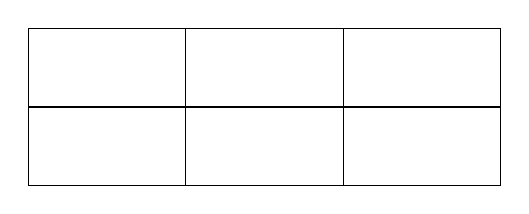
\begin{tikzpicture}
                \draw (0, 0) -- (6, 0) -- (6, 2) -- (0, 2) -- cycle;
                \draw (0, 1) -- (6, 1);
                \draw (2, 0) -- (2, 2);
                \draw (4, 0) -- (4, 2);
            \end{tikzpicture}
        \end{center}
        \vspace{3cm}
    \item If $99$ people stand in a circle, and each skaes the hand of the 
		person on each side, how many handshakes are there all together?
		\vspace{3cm}
\end{enumerate}

\end{document}